% !TeX TS-program = xelatex
% This is SJTUBeamermin v1.0
% For more detailed desciption, see
% https://github.com/LogCreative/SJTUBeamermin/blob/main/doc/sjtubeamermintheme.pdf
%
\documentclass[
    % draft,                             % 草稿模式
    aspectratio=169,                   % 使用 16:9 比例
]{beamer}
\mode<presentation>
\usetheme[
    navigation=subsections,            % 使用子章节进度显示
     lang=en,                           % 使用英文
    % cjk=true,                          % 使用CJK而不是ctex
    color=blue,                         % 使用红色主题
    % pattern=all,                        % 使用全图案装饰
    % gbt=bibtex,                        % 使用 gbt (使用 bibtex 编译)
]{sjtubeamermin}
% \usecolortheme[]{beaver}                 % 使用其他颜色主题
% \addbibresource{ref.bib}               % gbt!=bibtex

\usepackage{amsmath,amssymb,amsthm}
\usepackage{bm}
\usepackage{xcolor}
\usepackage{tikz-cd}
\usepackage{tikz}
\usetikzlibrary{trees}
\usepackage{empheq}
\usepackage{tabularx}
\usepackage{multicol}
\usepackage[linesnumbered,ruled]{algorithm2e}
\usepackage{hyperref}
\usepackage{amsfonts}
\usepackage{fontspec}
\usepackage{mdframed} % Add easy frames to paragraphs
\usepackage{color,soul}
\usepackage{xparse} % Add support for \NewDocumentEnvironment
\renewcommand{\Bbb}{\mathbb}
\newcommand{\Z}{\mathbb{Z}}
\newcommand{\GR}{\mathbb{GR}}
\newcommand{\F}{\mathbb{F}}
\newcommand{\R}{\mathbb{R}}
\newcommand{\Fn}{\mathbb{F}_2^n}
\newcommand{\Fm}{\mathbb{F}_2^m}
\newcommand{\df}{\delta_F}
\newcommand{\tr}{\operatorname{tr}}
\newcommand{\gtr}{\operatorname{T}}
\newcommand{\teich}{\textit{Teichm$\ddot{u}$ller sets}}
% \newtheorem*{definition}{Definition}
\newtheorem{thm}{Theorem}
\newtheorem{lem}[thm]{Lemma}
\newtheorem{proposition}{Proposition}
\definecolor{graylight}{cmyk}{.30,0,0,.67} % define color using xcolor syntax
\setbeamertemplate{itemize items}[default]

\newmdenv[ % Define mdframe settings and store as leftrule
  linecolor=red,
  topline=false,
  bottomline=false,
  rightline=false,
  skipabove=\topsep,
  skipbelow=\topsep
]{leftrule}

% \NewDocumentEnvironment{example}{O{\textbf{Example:}}} % Define example environment
% {\begin{leftrule}\noindent\textcolor{blue}{#1}\par}
% {\end{leftrule}}
\setbeamertemplate{footline}[frame number]

\NewDocumentEnvironment{question}{O{\textbf{Something:}}} % Define something environment
{\begin{leftrule}\noindent\textcolor{graylight}{#1}\par}
{\end{leftrule}}

\NewDocumentEnvironment{remark}{O{\textbf{Remark:}}} % Define remark environment
{\begin{leftrule}\noindent\textcolor{blue}{#1}\par}
{\end{leftrule}}

\begin{document}
    \institute[School of Electronic Information and Electrical Engineering]{电子信息与电气工程学院}   % 组织
    % \logo{
    %     
\includegraphics{support/cnlogored.pdf}  % 重定义 logo
    % }
    \titlegraphic{                         % 标题图像
        \begin{stampbox}[white]
            
\includegraphics[width=0.3\textwidth]{support/head.png}
        \end{stampbox}
    }
    \title{APN functions}  % 标题
 %   \subtitle{SJTUBeamer \fbox{\textsc{min}} Template}         % 副标题
    \author{Zhaole Li}                  % 作者
    \date{\textcolor{red}{Workshop of APN function, 2022}}                          % 日期
    \maketitle                             % 创建标题页


\AtBeginSection[]{
    \begin{frame}
        % \tableofcontents[currentsection]           % 传统节目录             
        \sectionpage                   % 节页
    \end{frame}
}

% 使用小节目录
%\AtBeginSubsection[]{                  % 在每小节开始
 %   \begin{frame}
        % \tableofcontents[currentsection,currentsubsection]             % 传统小节目录             
  %      \subsectionpage                % 小节页
 %   \end{frame}
%}

\section{Introduction}
%\subsection{第 1 小节}

    \begin{frame}
        \frametitle{Vectorial Boolean functions}
    
        Given two positive integers $n$ and $m$, a vectorial Boolean $(n, m)$-function, or simply $(n, m)$-function, is any function $F:\F_2^n\rightarrow\F^m_2$.
        When $ m=1 $, we often call it $ n $-variable Boolean function. 
        
        One can identify the vector space $ \F_2^n $ with the finite field $ \F_{2^n} $.

    \end{frame}
    \begin{frame}
        \frametitle{Walsh transform of Boolean functions}
        
        For a given $n$-variable pseudo-Boolean function $ \varphi $, which is a function from $\F^n_2$ to $\R$, the Fourier-Hadamard transform of $ \varphi $
        defined on $ \F_2^n $ by:
        \[\hat{\varphi}(u)=\sum_{x\in\F_2^n}\varphi(x)(-1)^{u\cdot x},u\in\F_2^n,\]
        where ``$\cdot$'' is the inner product in $ \F_2^n $ such as $ u\cdot x=\sum_{i=1}^{n}u_ix_i $. 

        For a given $n$-variable Boolean function $ f $, set $ \varphi=(-1)^f $, then we obtain the Walsh transform of $f$:
        \[ W_f(u)=\sum_{x\in\F_2^n}(-1)^{f(x)+u\cdot x},u\in\F_2^n.\]
        The two transforms are related by $ W_f(u)=2^n\delta_0(u)-2\hat(f)(u) $, where $ \delta_0 $ is the Dirac symbol.
        
    \end{frame}

    \begin{frame}
        \frametitle{Walsh transform of Boolean functions}
    
        Parseval relation:
        \[\sum_{u\in\F_2^n}W_f^2(u)=2^{2n}.\]
        Titsworth relation:
        \[\sum_{u\in\F_2^n}W_f(u)W_f(u+v)=0,v\neq 0.\]
    
    \end{frame}

    \begin{frame}
        \frametitle{The nonlinearity of a (vectorial) Boolean function}
    
        The nonlinearity of a Boolean function $f$ equals its minimal Hamming distance to affine Boolean functions $u \cdot x + \epsilon$,
         where $ u\in\F_2^n,\epsilon\in\F_2 $:
        \[nl(f)=2^{n-1}-\frac{1}{2}\max_{u\in\F_2^n}|W_f(u)|.\]
        The nonlinearity of an $(n, m)$-function $F$ equals the minimal nonlinearity of its component functions $v \cdot F$, where $v \in \F^m_2\setminus\{0_m\}$:
        \[nl(F)=2^{n-1}-\frac{1}{2}\max_{\substack{u\in\F_2^n\\v\in\F_2^m,v\neq 0_m}}|W_F(u,v)|\footnote{The Walsh transform of an $(n, m)$-function is defined in terms of the Walsh transform of its component functions: $ W_F(u,v)=\sum_{x\in\F_2^n}(-1)^{v\cdot F(x)+u\cdot x},v\neq 0 $.}.\]
    \end{frame}


    \begin{frame}
        \frametitle{Differential uniformity}
        The differential attack, introduced by Biham and Shamir\footnote{E. Biham and A. Shamir. Differential cryptanalysis of DES-like cryptosystems. Journal of
        Cryptology 4 (1), pp. 3–72, 1991.}, is a chosen plaintext attack for block ciphers in general.

        An $(n,m)$-function $F$ is called differentially $\delta$-uniform, if for every nonzero $a \in \Fn$ and every $b\in\Fm$, 
        the equation $F(x)+F(x+a)=b$ has at most $\delta$ solutions. We denote the minimum of these integers $ \delta $ by $ \delta_F $
        and call it the differential uniformity of $F$. For every $(n, m)$-function $F$, we have $\delta_F \geq \max(2, 2^{n−m})$.
    \end{frame}
    \begin{frame}
        \frametitle{APN functions}
        We can have $\delta_F = 2$ only when $n \geq m$, and this case is specially defined for $ n=m $:
        \begin{definition}[APN functions]
            An $(n, n)$-function $F$ is called almost perfect nonlinear (APN) if it is differentially $2$-uniform, i.e.
            if for every $a \in \Fn \setminus \{0_n\} $ and every $b \in \Fn$, the equation $F(x) + F(x + a) = b$ has $0$ or $2$ solutions 
            (i.e. the derivative $D_aF(x) = F(x) + F(x + a)$ is $2$-to-$1$). Equivalently, $|{D_aF(x), x \in \Fn}| =2^{n−1} $.
            In other words, for distinct elements $x, y, z, t\in\Fn$, the equality $ x + y + z + t = 0_n $ implies $F(x) + F(y) +F(z) + F(t) \neq 0_n$. 
        \end{definition}
    \end{frame}


    % \begin{frame}
    %     \frametitle{Introduction}
    %     \begin{itemize}
    %         \item The differential uniformity $ \df $ is even since the solutions of equation 
    %         $ F(x)+F(x+a)=b $ come out by pairs: if $ x  $ is the solution, then $ x+a $ is also a solution.
    %         \item Lower differential uniformity means better resistance to the differential attack
    %         \item The low bound of differential uniformity $ \df $ of any $ (n,m) $ function $ F $ is $ 2^{n-m} $
    %         \item The differential uniformity equals $2^{n−m}$ if and only if every derivative $D_aF, a \neq 0$, is balanced, and we say $F$ is perfect nonlinear
    %     \end{itemize}
    % \end{frame}
\section{The distance between APN functions\footnote{Budaghyan L, Carlet C, Helleseth T, et al. On the distance between APN functions[J]. IEEE Transactions on Information Theory, 2020, 66(9): 5742-5753.}}
    \begin{frame}
        \frametitle{The distance between APN functions}
    
        Given two functions $F,G:\F_2^n \rightarrow \F_2^n$, the Hamming distance $d(F, G)$ is defined as the number of points $ x \in \F_2^n $  which the
        values of $F(x)$ and $G(x)$ differ, i.e. 
        \[d(F, G) = |\{x \in\F_2^n : F(x) \neq G(x)\}|.\]
    
        Hence, we consider the case of arbitrarily changing the values of $ K $ points, obviously the Hamming distance $ d(F,G)=K $. 
        In fact, given a function $F : \F_2^n \rightarrow \F_2^n$, 
        $K$ distinct elements $u_1,u_2,\dots,u_K \in \F_2^n$ and the corresponding $K$ elements $v_1,v_2,\dots,v_K \in \F_2^{n}\setminus\{0_n\}$, we define $G$ as
        \[G(x)=\left\{\begin{aligned}
            &F(u_i)+v_i, x=u_i\\
            &F(x), x\notin\{u_1,u_2,\dots,u_K\}.
        \end{aligned}\right.\]
    \end{frame}

    \begin{frame}
        \frametitle{The derivative of function G}
    
        We define the indicator function of a set $ S $: $ 1_S(x)=\left\{\begin{aligned}
            &1,&~if~x\in S\\
            &0,&~otherwise.
        \end{aligned}\right. $

        Therefore the function $ G $ defining over $ F $ can be written as 
        \[G(x)=F(x)+\sum_{i=1}^{K}1_{u_i}(x)v_i=F(x)+\sum_{i=1}^{K}(1+(x+u_i)^{2^n-1})v_i.\]

        So we can observe that for any $ a\in\F_2^n\setminus\{0_n\} $, the derivative $ D_aG $ takes the form
        \[D_aG(x)=D_aF(x)+\sum_{i=1}^{K}1_{u_i}(x)v_i=D_aF(x)+\sum_{i=1}^{K}1_{u_i,a+u_i}(x)v_i.\] 
    \end{frame}
    
    \begin{frame}
        \frametitle{The derivative of function G}
    
        Denote $ U=\{u_1,u_2,\dots,u_K\} $ is the set of points which values of function $ F $ will change. Denote $ a+U $ by the set $ \{a+u\mid u\in U\} $.
        It's possibe that there exist $ 1\leq i,j\leq K $ such as $ u_j=a+u_i $, leading to the two $ v_i,v_j $ appearing in the $ D_aG(u_i) $.
        Thus denote $ U_a $ by the set $ \{u\in U\mid u\in a+U \} $, $ \overline{U_a}=U\setminus U_a $. For convenient, we define a function $ p_a $ on
        the index of of $ U $ by $ p_a(i)=j $ where $ j $ satisfies $ u_j=a+u_i $.
        
        So the equation $ D_aG $ can be written more easily in the form
        \[D_aG(x)=D_aF(x)+\sum_{u_i\in U_a,i<p_a(i)}1_{u_i,u_{p_a(i)}}(v_i+v_{p_a(i)})+\sum_{u_i\in\overline{U_a}}1_{u_i,a+u_i}(x)v_i.\]
    
    \end{frame}

    \begin{frame}
        \frametitle{When G is an APN function}
    
        $ G $ is an APN function iff $ D_aG $ is $ 2 $-to-$ 1 $, which means for $ a\in\F_{2^n}^* $, $ D_aG(x)=D_aG(y) $ occurs for $ x=y $ or $ x=y+a $.

        \begin{theorem}
            Let $ F : \F_{2^n} \rightarrow \F_{2^n} $, let $ u_1, u_2, \dots , u_K $ be $K$ distinct points from $\F_{2^n}$ and let $ v_1, v_2, \dots , v_K $ be $K$ arbitrary elements from $ \F_{2^n}^* $. Then function $ G $ is APN if all of the following conditions are satisfied for all $ a\in\F_{2^n}^* $:
            \begin{enumerate}
                \item[(i)] $ D_aF $ is $ 2 $-to-$ 1 $ on $ \F_{2^n}\setminus (U\cup a+U) $;
                \item[(ii)] $D_{a} F(u_{i})+D_{a} F(u_{j}) \neq v_{i}+v_{j}+v_{p_{a}(i)}+v_{p_{a}(j)}$ for $u_{i}, u_{j} \in U_{a}$ unless $u_{i}=u_{j}$ or $u_{i}+u_{j}=a$;
                \item[(iii)] $D_{a} F\left(u_{i}\right)+D_{a} F\left(u_{j}\right) \neq v_{i}+v_{j}+v_{p_{a}(i)}$ for $u_{i} \in U_{a}, u_{j} \in \overline{U_{a}}$;
                \item[(iv)] $D_{a} F\left(u_{i}\right)+D_{a} F\left(u_{j}\right) \neq v_{i}+v_{j}$ for $u_{i}, u_{j} \in \overline{U_{a}}$ unless $u_{i}=u_{j}$;
                \item[(v)]  $D_{a} F\left(u_{i}\right)+D_{a} F(x) \neq v_{i}+v_{p_{a}(i)}$ for $u_{i} \in U_{a}, x \notin(U \cup a+U)$;
                \item[(vi)] \fcolorbox{red}{yellow}{$D_{a} F\left(u_{i}\right)+D_{a} F(x) \neq v_{i}$ for $u_{i} \in \overline{U_{a}}, x \notin(U \cup a+U)$.}
            \end{enumerate}
        \end{theorem}
    
    \end{frame}

    \begin{frame}
        \frametitle{Proof by contrapositive}
    
        We prove it by contrapositive: assume there is a tuple $ (a,x,y)\in\F_{2^n}^*\times\F_{2^n}^2 $ with $ x\neq y,x\neq a+y $ satisfying $ D_aG(x)=D_aG(y) $.
        Since $ D_aG(x) $ has three cases for $ x $ in $ \overline{U_a},U_a $ or $ \F_{2^n}\setminus(U\cup a+U) $, we must run over 
        all possible cases for $ (a,x,y) $. 
        \[\left\{
            \begin{aligned}
                &x,y\in(U\cup a+U)\\
                &x,y\notin(U\cup a+U)\left\{\begin{aligned}
                    &x,y\in U_a\\
                    &\text{one of }~x,y\in U_a\\
                    &x,y\notin U_a
                \end{aligned}\right.\\
                &\text{one of }~x,y\in(U\cup a+U)\left\{\begin{aligned}
                    x\in U_a\\
                    x\in\overline{U_a}
                \end{aligned}\right.\\
            \end{aligned}
        \right.\]
    
    \end{frame}

    \begin{frame}
        \frametitle{Proof by contrapositive}
        \begin{itemize}
            \item Consider the first case, when $ x,y\notin(U\cup a+U) $, we have $ D_aF(x)=D_aF(y) $, so we confirm that $ D_aF $ cannot be $ 2 $-to-$ 1 $ over
            $ \F_{2^n}\setminus(U\cup a+U) $ since $ x\neq y,x\neq a+y $. Conversely, if $ D_aF $ is $ 2 $-to-$ 1 $ over $ \F_{2^n}\setminus(U\cup a+U) $,
            it's easy to see that there exists no tuple $ (a,x,y) $ satisfying the 
            
            \item Consider the last case, assume $ D_aG(u_i)=D_aG(y) $ for $ u_i=x\in\overline{U_a} $ and $ y\notin(U\cup a+U) $, we have 
            $ D_aF(u_i)+v_i=D_aF(y) $. So we arrive at (vi).
        \end{itemize}

    \end{frame}

    \begin{frame}
        \frametitle{Fixed points $ u_1,u_2,...,u_K $}
    
        By fixing the function $ F $ with $ K $ points $ u_1,u_2,\dots,u_K $, we can reduce the number of potential values for the values $ v_1,v_2,\dots,v_K $.
        \begin{algorithm}[H]
            \SetKwInOut{Input}{Input}
            \SetKwInOut{Output}{Output}
            \Input{The set of $ K $ distinct points $ U=\{u_1,u_2,\dots,u_K\}\subseteq\F_{2^n} $ with a function $ F:\F_{2^n}\rightarrow\F_{2^n} $.}
            \Output{A domain $ D_i\subseteq\F_{2^n} $ for all $ v_i $ s.t. if $ G $ is APN, then $ v_i\in D_i $ for all $ i $.}
            \For{$i\leftarrow 1 $ \KwTo $ K $}{
            set $D_i$ $\leftarrow$ $\F_{2^n}$\;
            compute $A$ $\leftarrow$ $\{D_aF(x)+D_aF(u_i):x,a\in\F_{2^n},a\neq 0,u_i\in\overline{U_a},x\notin(U\cup a+U)\}$\;
            update $D_i$ $\leftarrow$ $ D_i\setminus A$\;
            }
            \caption{Reducing the domains of $ v_i $}
        \end{algorithm}
    \end{frame}

    \begin{frame}
        \frametitle{Example}
        \parindent0em
        \begin{multicols}{2}[\columnsep2em] 
            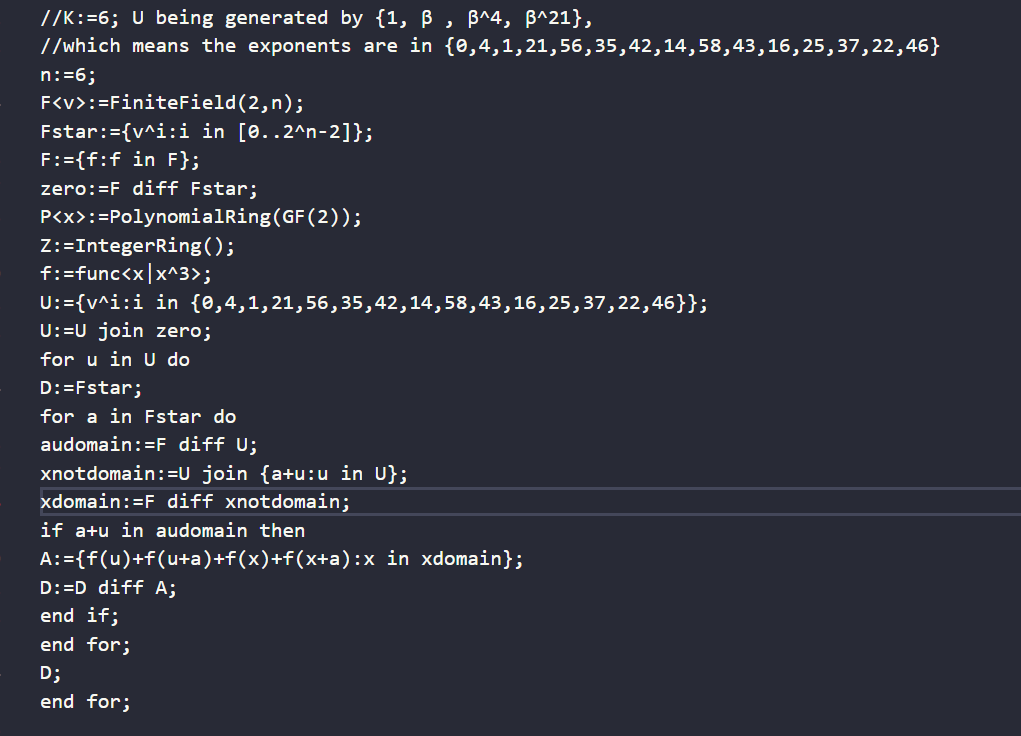
\includegraphics[width=\linewidth]{code_image.png}
            \columnbreak

            {Take $ F(x)=x^3 $ over $ \F_{2^6} $ with $ U $ generated by $ \{1,\beta,\beta^4,\beta^{21}\} $ in the sense of additive closure with $ \beta $ is primitive in $ \F_{2^6} $. We get the result}
            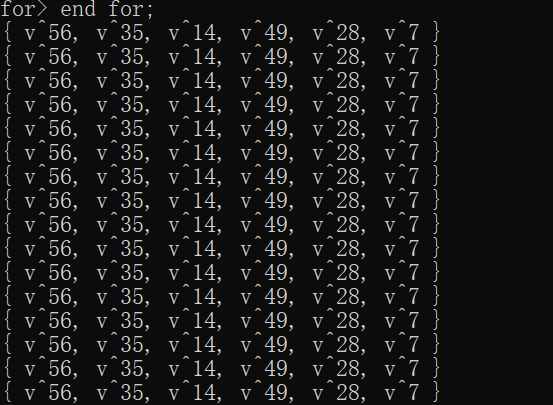
\includegraphics[width=0.8\linewidth]{code_result.png}
        \end{multicols}

    
    \end{frame}

    \begin{frame}
        \frametitle{Example}
    
        In above situation (when the set of points $U$ can be transformed into an APN function), the filtering procedure
        may leave rather large domains for the candidates, which still needs long computations: the $ 6^{16} $ potential candidates are left to be examined, 
        and actually there are only $ 6 $ possible candidates that lead to an APN function, which are all the same values for the $ 16 $ points.
        So there are still many things to impose on the values $ v_i $. 

        But in some cases (when the set of points $ U $ cannot be transformed into an APN function), no values are left for some $ v_i $, which implies no APN
        functions can be obtained by changing the values in the points $ U $ of $ F $.
    \end{frame}

    \begin{frame}
        \frametitle{The property between $ F $ and $ G $}
    
        When both $ F $ and $ G $ are APNness, we can get the following property for the distance between $ F $ and $ G $:
        \begin{corollary}
            Let $F$ and $G$ be as in the statement of Theorem 1 with $v_i \neq 0$ for $1\leq i \leq K$, and assume, in addition, that $F$ is APN;
            consider some fixed $ i $, then no more than $3(K−1)$ derivatives of the form $D_a F(x)+F(u_i+a)$ map to $G(u_i)$. 
        \end{corollary}
    
    \end{frame}

    \begin{frame}
        \frametitle{Proof}
        
        In theorem 1 (vi), if $ G $ is an APN, then $ D_aF(u_i)+D_aF(x)\neq v_i $ for $ u_i\in\overline{U_a},x\notin(U\cup a+U) $, 
        i.e. $ F(u_i+a)+D_aF(x)\neq F(u_i)+v_i=G(u_i) $ for $ u_i\in\overline{U_a},x\notin(U\cup a+U) $. This equation gives some insight of 
        the property between $ G $ and $ F $:
        \begin{itemize}
            \item when $ x\in(U\cup a+U) $,  there are chances that $ F(u_i+a)+D_aF(x)=G(u_i) $ for $ u_i\in\overline{U_a} $, 
            and the number of solution is at most $ 2(K-1) $ since $ U\cap a+U\neq\emptyset $;
            \item when $ x\in(U\cup a+U) $ and $ u_i\in U_a $, we confirm that there are at most $ K $ such direction $ a $, but note that 
            $ a\neq 0 $, so there are at most $ K-1 $ direction $ a $.
        \end{itemize}
    \end{frame}

    \begin{frame}
        \frametitle{Corollary}
        \begin{corollary}
            
            Let $F$ be an APN function over $\F_{2^n}$ and let $m_F$ be the number 
            \[m_F=\min_{b,\beta\in\F_{2^n}}\lvert\Pi_F^{\beta}(b)\rvert\footnote{we define $ \Pi_F^{\beta}(b) $ to be the set of derivative directions $a$ for which $D_aF(x)+F(\beta+a)$ maps to $b$, i.e. 
            \[\Pi_F^{\beta}(b)=\{a\in\F_{2^n}:D_aF(x)+F(\beta+a)=b~\text{has solutions}\}.\]}.\]
            Then for any APN function $G \neq F$ over $\F_{2^n}$, the Hamming distance $d(F, G)$ between $F$ and $G$ satisfies
            \[d(F,G)\geq\lceil\frac{m_F}{3}\rceil+1.\]
        \end{corollary}
    
    \end{frame}

    \begin{frame}
        \frametitle{Proof of the Corollary}
    
        From above we conclude if two APN functions $ F,G $ have distance $ K $, then we can compute all possible values $ D_aF(x)+F(u_i+a) $
        for $ u_i $ and $ G(u_i) $.  
        Therefore when $ b,\beta $ run over $ \F_{2^n} $, we compute a series of $ \Pi_F^{\beta}(b) $,
        whose cardinalities must have the minimal value, which is $ m_F $.
        Of course $ m_F\leq 3(K-1) $, so we arrive at the corollary.

    \end{frame}
\section{The lower bound of nonlinearity for known APN functions\footnote{Carlet C. On the properties of the Boolean functions associated to the differential spectrum of general APN functions and their consequences[J]. IEEE Transactions on Information Theory, 2021, 67(10): 6926-6939.}}
    \begin{frame}
        \frametitle{The Boolean function $ \gamma_F $}
    
        We can define $ \gamma_F(a,b) $ as below:
        $ \forall a,b\in\F_2^n,\gamma_F(a,b)= $
        \[\left\{\begin{aligned}        
            &1, ~\text{if} ~a\neq 0_n~\text{and}~ F(x)+F(x+a)=b ~\text{has~solutions}\\
            &0, ~\text{otherwise}.
        \end{aligned}\right.\]

        Thus, for every APN $ (n,n) $-function $ F $, we view it as a Boolean function
        $ \frac{|(D_aF)^{-1}(b)|}{2}-2^{n-1}\delta_0(a,b) $, then we have 
        \[\widehat{\gamma_F(u,v)}=\frac{1}{2}W_F^2(u,v)-2^{n-1}.\]
        So we confirm that for every $ u,v $:
        \[W_{\gamma_F}(u,v)=\left\{\begin{aligned}
            &2^n, ~\text{if}~ v=0_n\\
            &2^n-W_F^2(u,v), ~\text{if}~ v\neq 0_n.
        \end{aligned}\right.\]
        
    \end{frame}   

    \begin{frame}
        \frametitle{The Walsh transform of the APN function}
    
        The fourth moment of the Walsh transform of an APN function $ F $:
        \[\sum_{u,v\in\F_2^n}^{}W_F^4(u,v)=3\cdot 2^{4n}-2^{3n+1}.\]
        When apply the Titsworth relation on the $ \gamma_F $, we have for all $ (u_0,v_0)\neq(0_n,0_n) $,
        \[\sum_{u,v\in\F_2^n}^{}W_{\gamma_F}(u,v)W_{\gamma_F}(u+u_0,v+v_0)=0.\]
        Then we have the following theorem:
        
    
    \end{frame}
        
    \begin{frame}
        \frametitle{The lower bound of nonlinearity for known APN functions}
        \begin{theorem}
            Any APN $ (n,n) $-function $ F $ satisfies that  for all $ (u_0,v_0) $,
            \[\sum_{\substack{u,v\in\F_2^n\\v\neq 0_n,v\neq v_0}}W_F^2(u,v)W_F^2(u+u_0,v+v_0)=2^{4n}-2^{3n+1}+2^{4n}\delta_0(u_0,v_0).\] 
        \end{theorem}
        \begin{corollary}
            If there exists $ (u_0,v_0)\neq(0_n,0_n) $ such that $ |W_F(u,v)| $ and $ |W_F(u+u_0,v+v_0)| $ 
            both achieve the maximun value of $ \{|W_F(u,v)|:u,v\in\F_2^n;v\neq 0_n\} $, 
            then we have 
            \[nl(F)\geq 2^{n-1}-\frac{1}{2}\sqrt[4]{2^{4n-1}-2^{3n}}.\]
        \end{corollary}
    
    \end{frame}
    \makebottom     % 创建尾页  % 非标准命令

\end{document}